\chapter{PELAKSANAAN PENELITIAN}
\label{pelaksanaan-penelitian}

\section{Alat dan Bahan Penelitian}
Penelitian ini tidak dapat dilakukan tanpa adanya alat dan bahan yang memudahkan penulis dalam melakukan penelitian. Alat dan bahan yang digunakan oleh penulis disebutkan secara rinci pada Tabel \ref{tbl:4:alatbahan}, dan Tabel \ref{tbl:4:speklaptop}.

%\vspace{2em}
\begin{table}[!h]
	\caption{Daftar alat dan bahan}
	\label{tbl:4:alatbahan}
	\centering
	% use packages: array
	\begin{tabular}{|c|p{5cm}|p{8cm}|}
		\hline
		No. & Nama alat/bahan & Fungsi \\
		\hline
		1 & Laptop ASUS N550JX & Perangkat komputer perancangan jaringan saraf tiruan. \\
		\hline
		2 & Python versi 3.7 & Bahasa pemrograman. \\
		\hline
		3 & Visual Studio Code versi 1.38 & Aplikasi penulisan dan penyuntingan kode sumber. \\
		\hline
		4 & Jupyter Notebook 1.0 & Aplikasi web untuk menulis kode program, teks, persamaan, dan visualisasi. \\
		\hline
		5 & Scikit-Learn versi 0.21 & Pustaka pembangunan jaringan saraf tiruan. \\
		\hline
		6 & IES-VE 2019 & Perangkat lunak untuk pengambilan data lingkungan termal \textit{climate chamber} dan variasi gangguan. \\
		\hline
		7 & MS Excel 365 & Perangkat lunak pengolahan data tabular. \\
		\hline
		8 & MATLAB R2016a & Perangkat lunak untuk menjalankan simulasi sistem kontrol. \\
		\hline
		%6 & Raspberry Pi versi 3 B & Komputer mikro sebagai perangkat pengendali. \\
		%\hline
	\end{tabular}
\end{table}

%\vspace{2em}
\begin{table}[!h]
	\caption{Spesifikasi laptop ASUS N550JX}
	\label{tbl:4:speklaptop}
	\centering
	% use packages: array
	\begin{tabular}{|c|p{5cm}|p{8cm}|}
		\hline
		No. & Komponen & Spesifikasi \\ 
		\hline
		1 & Processor & Intel Core i7-4720HQ CPU @ 2.60GHz x 8 \\ 
		\hline
		2 & Graphics & Intel Haswell Mobile \\
		\hline
		3 & RAM & 8 GB \\ 
		\hline
		4 & Tipe sistem operasi & 64-bit \\
		\hline
		5 & Sistem operasi & Manjaro Linux \\ 
		\hline
	\end{tabular}
\end{table}

\section{Tata Laksana Penelitian}
Alur penelitian yang digunakan penulis dalam mencapai tujuan dapat dilihat pada Gambar \ref{fig:4:TataLaksanaPenelitian} berikut.
\begin{figure}[!h]
	\centering
	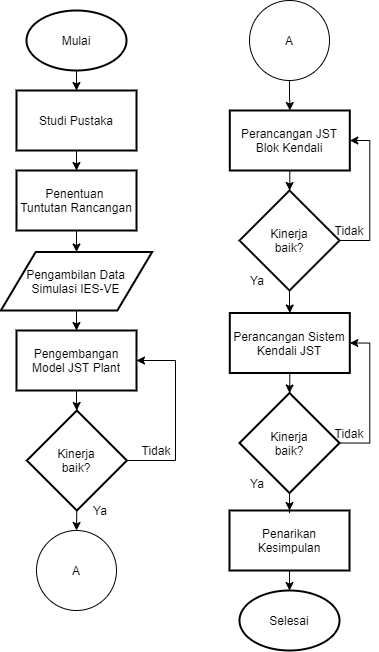
\includegraphics[width=0.3\textwidth]{figures/TataLaksanaPenelitian}
	\caption{Bagan Tata Laksana Penelitian}
	\label{fig:4:TataLaksanaPenelitian}
\end{figure}

%\begin{figure}[!h]
%	\centering
%	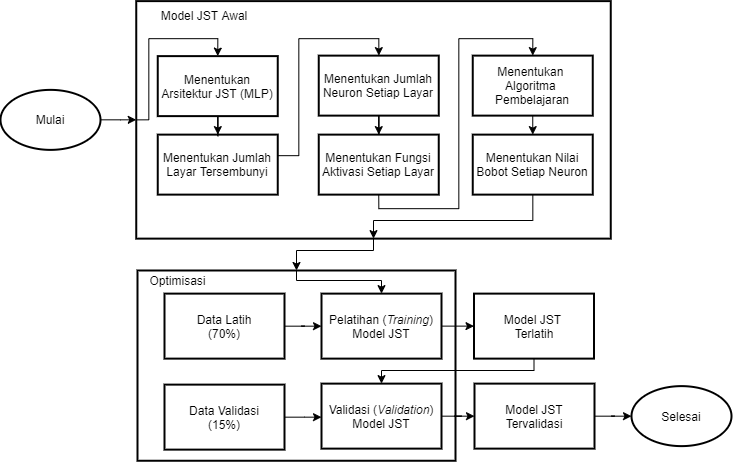
\includegraphics[width=0.85\textwidth]{figures/PerancanganModel}
%	\caption{Bagan Perancangan Model JST}
%	\label{fig:4:DiagramPerancanganModel}
%\end{figure}

%\begin{landscape}
%	\begin{figure}[!h]
%		\centering
%		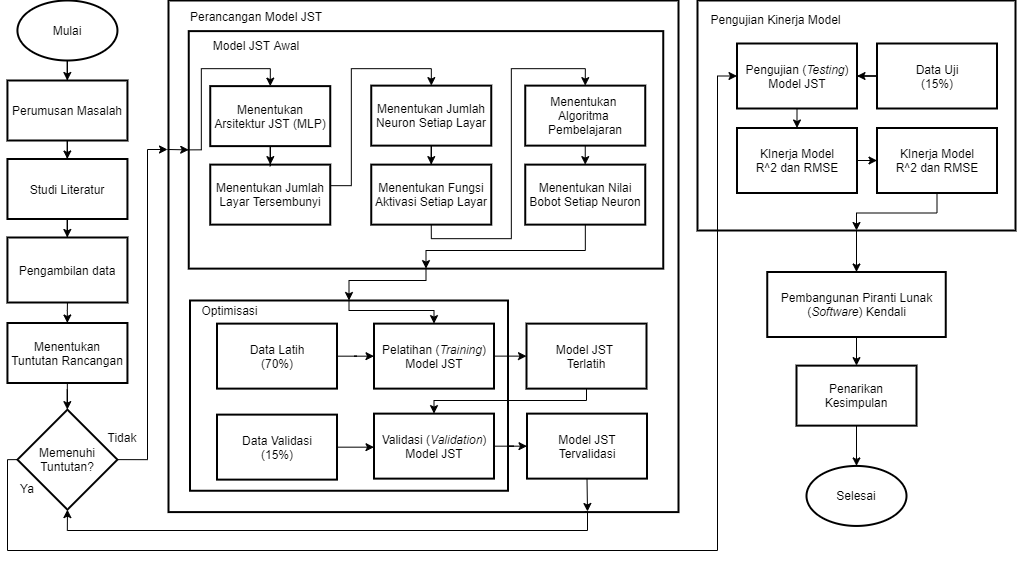
\includegraphics[width=1.5\textwidth]{figures/DiagramPenelitianFull}
%		\caption{Diagram Alir Penelitian Utuh}
%		\label{fig:4:DiagramPenelitianFull}
%	\end{figure}
%\end{landscape}

\subsection{Studi Literatur}
Studi literatur bertujuan untuk mendapatkan pemahaman dalam penyelesaian masalah yang diangkat dalam penelitian ini. Studi literatur juga membantu menegaskan tujuan penelitian sehingga penulis mampu mengetahui perbedaan penelitian ini dengan penelitian terkait yang telah dilakukan sebelumnya. Dari studi literatur yang telah dilakukan maka akan memperjelas tuntutan perancangan dari sistem yang akan dibuat. Informasi yang digunakan bersumber dari berbagai artikel ilmiah, jurnal, skripsi, buku, dan/atau sumber tertulis lainnya yang membahas mengenai sistem kendali lingkungan termal dan/atau jaringan saraf tiruan.

\subsection{Penentuan Tuntutan Rancangan}

Tuntutan pada rancangan ini merujuk pada standar SNI dengan nilai standar suhu udara dijaga pada nilai 25 $\pm$ 1$^{\circ}$C dan nilai kelembapan dinyatakan dalam bentuk \textit{relative humidity} (RH), dijaga pada nilai 60\% $\pm$ 10\%. Sehingga dapat dikatakan bahwa \textit{setpoint} untuk suhu udara bernilai 25$^{\circ}$C dan untuk kelembapan udara (RH) sebesar 60\% dengan kesalahan keadaan tunak tidak melebihi 1$^{\circ}$C (suhu udara) dan 10\% (kelembapan relatif) \cite{SNI-03-06390-2000}. Nilai tersebut akan digunakan sebagai acuan untuk menganalisis perbedaan suhu udara dan kelembaban relatif antara data target dan data prediksi.

\subsection{Pengambilan Data Simulasi IES-VE}
Penelitian ini menggunakan data dari model yang telah dibuat di penelitian sebelumnya berjudul \textbf{Karakterisasi Lingkungan Termal Chamber Iklim Menggunakan Metode Simulasi CFD dengan Perangkat Lunak IES-VE} yang diteliti oleh Ichfan Kurniawan \cite{skripsiIchfan}.  Data tersebut merupakan hasil simulasi pada \textit{software} IES-VE dengan menerapkan beberapa variasi kondisi lingkungan pada model \textit{climate chamber}. Variasi tersebut yaitu kondisi batas lingkungan (radiasi matahari dan suhu bola kering luar / \textit{drybulb temperature}), kondisi AC, dan kondisi \textit{heater}. Variasi kondisi batas lingkungan tersebut diwujudkan dalam pembagian 4 musim dalam 1 tahun, yakni bulan maret, juni, september dan desember. Keluaran dari model IES-VE berupa nilai suhu udara ruang (\textit{air temperature}) \textit{chamber} dan kelembapan relatif (RH) \textit{chamber}. Dari model tersebut didapatkan nilai MAE perhitungan selisih variabel lingkungan termal hasil simulasi dan pengukuran lapangan sebesar 0,8 $\pm$ 0,7$^{\circ}$C untuk suhu udara dan 2,5 $\pm$ 3,8\% untuk kelembaban relatif \cite{skripsiIchfan}. Data yang sudah terkumpul disajikan dalam bentuk tabular yang kemudian diolah dalam program komputer yang dibuat oleh penulis.

\subsection{Pemodelan \textit{Plant}}
Penelitian ini menggunakan model \textit{plant} yang telah dirancang dari penelitian sebelumnya berjudul \textbf{Pemodelan Lingkungan Termal Sistem \textit{Climate Chamber} dengan Metode Jaringan Saraf Tiruan} yang diteliti oleh Tri Hartanto \cite{skripsiTanto}. Model tersebut merupakan hasil perancangan pada piranti lunak MATLAB dengan menggunakan perangkat NNtools. Model \textit{plant} tersebut memiliki nilai MAE perhitungan antara target dan prediksi sebesar 0,59$^{\circ}$C untuk suhu udara dan 5,44\% untuk kelembapan relatif. Akurasi JST sebesar 96,23\% untuk suhu udara dan 68,90\% untuk kelembapan relatif \cite{skripsiTanto}. Model \textit{plant} tersebut akan diadaptasi oleh penulis dalam melakukan perancangan kendali berbasi jaringan saraf tiruan.

\subsection{Perancangan Kendali Berbasis JST}
Langkah awal untuk melakukan pemodelan kendali yaitu mendefinisikan terlebih dahulu pasangan data input dan data output dari sistem kendali. Untuk mendefinisikan nya perlu menyesuaikan variabel gangguan yang diberikan terhadap sistem dengan variabel keluaran dari AC yang dimana nilai keluaran tersebut dianggap optimal untuk menyesuaikan nilainya terhadap \textit{setpoint}. Nilai output tersebut didapat dari hasil simulasi pada software IES-VE, yang kemudian akan menjadi data latih pada JST yang digunakan pada software MATLAB. Adapun pasangan data kendali dilampirkan pada \textcolor{red}{Lampiran B}.

Pada langkah ini penulis menjabarkan variabel apa saja yang terlibat dalam \textit{plant} terkait sistem kendali yang akan dibuat. Dalam suatu sistem kendali perlu diketahui variabel apa saja yang termasuk dalam kategori \textit{controlled variables}, \textit{manipulated variables}, dan \textit{disturbance variables}. \textit{Controlled variables} adalah variabel akan dikendalikan dalam suatu sistem kendali. \textit{Manipulated variables} adalah variabel yang akan mempengaruhi nilai \textit{controlled variables} melalui \textit{manipulator}/\textit{actuator}. Sementara, \textit{disturbance variables} adalah variabel yang mempengaruhi sistem tetapi perancang tidak memiliki kuasa dalam mengatur nilainya. Hasil dari identifikasi sistem berbentuk diagram blok fungsional.

Untuk dapat mengetahui arsitektur JST dengan nilai error sekecil mungkin, dilakukan variasi arsitektur JST. Sama hal nya dngan pemodelan sistem, variasi yang dilakukan juga dengan memvariasikan jumlah layer tersembunyi, jumlah neuron dari masing-masing layer tersembunyi, serta fungsi aktivasi yang digunakan. Algoritma pembelajaran yang digunakan juga sama, yaitu dengan menggunakan Levenberg-Marquadt. Algoritma pembelajaran ini dianggap memiliki kecepatan pembelajaran yang tercepat, serta juga dianggap memiliki konvergensi terbaik untuk mencapai nilai mean square error (MSE) untuk masalah fungsi pendekatan suatu nilai tertentu [12] [13]. Parameter error yang digunakan juga sama, yaitu mean square error (MSE). Adapun proses training pada perancangan kendali juga memiliki proses yang sama dengan perancangan plant. Setelah didapat model yang dianggap baik, maka digunakanlah fungsi genism untuk membangun model di SIMULINK.

\subsection{{Penarikan Kesimpulan}}
Penarikan kesimpulan didapatkan berdasarkan hasil model terbaik yang terpilih dari beberapa percobaan variasi penentuan jumlah \textit{hidden layer} dan/atau jumlah neuron. Kesimpulan menggambarkan bagaimana parameter model yang terpilih sehingga dapat digunakan sebagai sistem kontrol lingkungan termal pada \textit{climate chamber} DTNTF FT UGM.

\section{Rencana Analisis Hasil Penelitian}
Data yang diperoleh dari hasil perancangan jaringan saraf tiruan berupa data nilai RMSE dari proses pelatihan, proses validasi, dan proses pengujian. Data nilai RMSE pengujian mewakili tingkat keakuratan model yang divariasikan. Semakin kecil nilai RMSE, semakin tinggi akurasi yang dihasilkan oleh model. Selain itu, tingkat konsistensi model juga perlu diuji dengan menggunakan nilai standar deviasi dari nilai \textit{error} pengujian. Model yang memiliki tingkat konsistensi yang tinggi merupakan model dengan standar deviasi \textit{error} paling rendah.

Model terpilih merupakan model yang memiliki tingkat akurasi dan konsistensi yang tinggi. Tingkat akurasi model dapat diwakili dengan nilai rerata RMSE pengujian. Sedangkan tingkat konsistensi diwakili dengan nilai standar deviasi RMSE pengujian terkecil. Semakin kecil nilai rata-rata dan standar deviasi RMSE pengujian, maka model yang dipilih semakin akurat dan konsisten.

Setelah penulis memilih model yang akurat dan konsisten, model tersebut diuji kinerjanya dengan cara membandingkan nilai prediksi dari model terhadap nilai target yang sebenarnya. Kemudian, pengujian model berlanjut dengan mengurangi keluaran jaringan yang akan diprediksi untuk melihat pengaruh jumlah keluaran jaringan terhadap \textit{error} yang dihasilkan.